\chapter{Evaluation}
This chapter deals with evaluating the results from the program when scoring article comparisons.

After having done tests to verify that the implementation of the algorithms worked correctly, it is now time to analyse the output.

\section{Scores}

The Cosine algorithm returns a score that is in fact an angle, where as the LCS algorithm returns a score that is based on the length of a string. As such these are hardly comparable in a one to one basis. If we modify the score of the LCS to not say something about the length of the substring(s), but tell us in percent how long the string is compared to the article is, it will produce a result that relates to the amount of text the two articles being compared have in common. This being said we still need to consider that the percentage value is relative to the length of the length of the article. We do therefore need to do a percentage calculation for both article's length. For better comparison of the Cosine and LCS score in the Excel graphs, the LCS percentage score is divided by 100 (even though comparing the scores is not really a decent indicator, it helps giving a better overview of the graphs).

So, a Cosine score of 1.0 means that the two article vectors are identical, same length and no angle between them. A LCS score of 1.0 means that the longest common substring's length is 100\% of the article's length. So each score will have to be evaluated on their own premisses, as a Cosine score of 0.5 is not 50\% identical. The Cosine score tells us something about how many special words that two articles have in common, where are the LCS tells us about the amount of text that is shared between the two articles.

\section{Limiting the Number of Comparisons by Cosine Score}

As discussed in the last chapter (see section ~\ref{AllFractiles}) there is many comparisons in the lowest fractile of the article comparisons. Although dismissing them right of the bat can be seen as hasty, the chance of comparisons scoring below 0.3 having much in common would be unlikely. This is because comparisons that score very low in the Cosine algorithm either have very little in common in terms of special words (as common words will have very little impact on the vector) or the article is very short and again, with few special words (we will see an example of this later on). However, an article with no special words that is very short, is very rare and few in between. We will however see examples of such articles later on.

For the sake of proving anything in this thesis how ever, and as the chance of getting useful results from comparisons with low Cosine scores are slim and the number of comparisons having to be humanly checked are massive in numbers should we check all comparisons, I will for the rest of this thesis, disregard all comparisons with a cosine score lower than 0.3.

\section{What the Scores Tell}
First off we need to realize what the different scores is telling us on their own. The cosine score will give an indication of how similar two articles are in regards to the words being used, but will not tell us anything in regards to what the article is actually saying in regards to the structure of sentences (see section ~\ref{CosineProblem}). By it's own, Cosine will tell us more about if the comparisons have the same topic that actually the same sentences. 

The modified LCS is an indication of how big a percentage of text in relation to article length that an article have in common with another article. The LCS score will therefore tell us a lot about how much actual text a comparison shares. 

\section{Score Analysis}

In figure ~\ref{SubstringsEx} we see a part of the LCS result of two articles being compared with each other. A long each axis we have an article (topmost row and leftmost column - not visible on image). The purple squares shows where a word match have been found, and a diagonal row of coloured squares indicate several words in concession have been found. If squares are coloured in purple, it means that the substring found is too short, if the squares are in brown the substring is equal to or greater than the threshold set for accepting substrings.

In the figure we see that the two articles start off with having a lot in common, then around two thirds into figure there is a huge gap along the x-axis, but it is largely unbroken along the y axis. So if judging the result by looking at this image we can establish two things.

\begin{itemize}
\item The two articles have a lot of text in common, but the article along the x-axis is substantially longer than the article along the y-axis.
\item The article along the y-axis is an excerpt of the article along the x-axis.
\end{itemize}

So when looking at this plot, we can tell if an article comparison is a duplicate, a excerpt or if there is no real match between two articles. To validate this fully it is needed to read the article text, to make sure the combination of substrings is not just a collection of random words, that are aligned in the same way without any relation.

In the following when looking at LCS comparison of articles, they are plotted like this in Excel. 

\section{Analysis of Comparisons}
In the following is described the evaluation of the scores produced by matching the four sources (JP being matched with POL and JV being matched with FL).

\subsection{JP and POL Comparison}
First off, the sources POL and JP was compared in the program. The results of this was then plotted in Excel (File: JPPOL.xlsx). The data columns are:

\begin{itemize}
\item \textbf{Left Id / Right Id:} The article Ids of the comparison. These are used to find the articles, when checking their content manually.
\item \textbf{Cosine Score:} The Cosine score for the comparison.
\item \textbf{LCS Score:} The unmodified LCS score. This is included for comparison with the modified LCS score. It is a percentage score off the longest of the two articles in the comparison.
\item \textbf{Combined Score Max:} The score from the modified LCS. This is a percentage score off the longest of the two articles in the comparison.
\item \textbf{Combined Score Min:} The score from the modified LCS. This is a percentage score off the shortest of the two articles in the comparison.
\item \textbf{Long Length:} The length of the longest article in characters.
\item \textbf{Short Length:} The length of the shortest article in characters.
\item \textbf{Match Group:} The match group the comparison have been placed into by the program (this will be explained later).
\item \textbf{Adjusted Score:} The score modification after applying score weighing (this will also be explained later).
\end{itemize}

Originally only the LCS score based off the longest article was included and used for evaluating the results. It did become clear after the first few tests, that this would not suffice. If we looked at two articles, one being substantially longer than the other, but the shortest being a 100\% excerpt of the longest, we could end up in a case where the article comparison would score very low because the LCS (and the Cosine for that matter) would be very low. We could then end up discarding this comparison as a "no match" because the scores was too low. How ever if we looked at the LCS score based off the length of the shortest article, we would get a completely different image. Then we could actually detect that the shortest article was in fact a excerpt, by seeing that it's LCS score would be 100\%. We will therefore have to look into the length of the articles as well, in order to fully say something about how much of a match a comparison is (this will be brought up again later).

Finally there are three graphs. The first is \textit{'Sample Distribution with Stopwords'}. This shows in a column diagram the comparisons different scores. As mentioned earlier we cannot compare the Cosine score with the LCS score on a one to one basis. However this does indicate something about general relations.

\begin{figure}
	\centering
	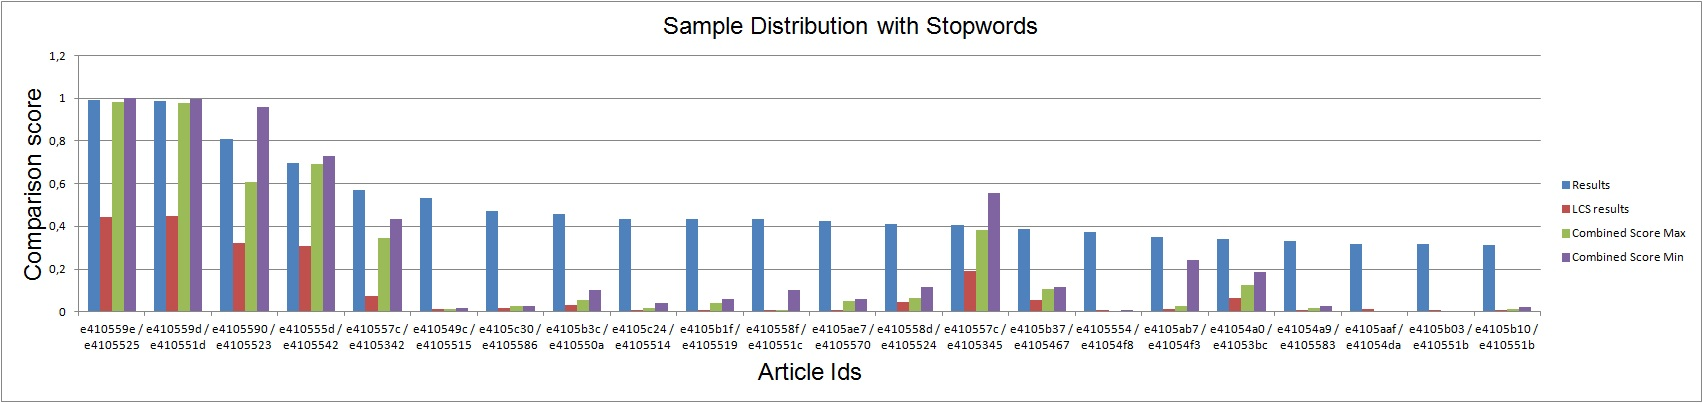
\includegraphics[scale=0.25]{figures/JPPOLScoreGraph}
	\caption{Comparison scores for the JP and POL sources (see appendix D for bigger image or File: JPPOL.xlsx).}
	\label{JPPOLScoreGraph}
\end{figure}

Figure ~\ref{JPPOLScoreGraph} shows the effect of having the modified LCS to collect all substrings longer than a given threshold. It also shows the necessity of having to evaluate the LCS score with both the length of the longest and the shortest article length as there can be quite a big difference in the scores.

Below that graph is two graphs side by side. The first shows the Cosine score plotted with the modified LCS score based off the longest article. The second graph shows the same, but this time the red dots is showing the Cosine and modified LCS score based off the shortest article.

The graphs in figure ~\ref{MaxScore} and ~\ref{MinScore} was created in order to get a better overview of how the scores was distributed. 

\begin{figure}
	\centering
	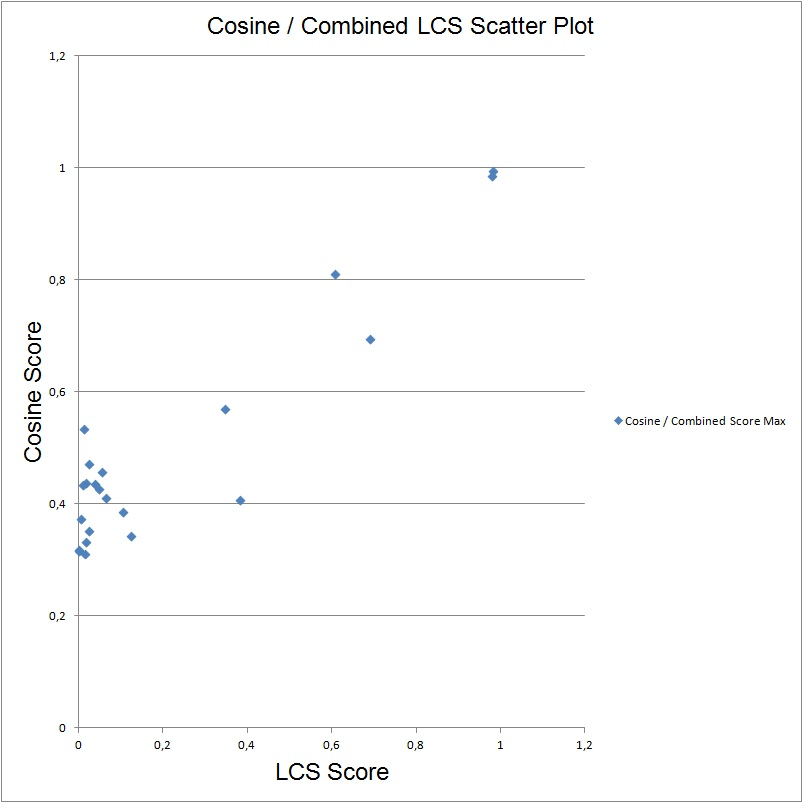
\includegraphics[scale=0.5]{figures/JPPOLCosineLCSMax}
	\caption{A plot showing the Cosine / LCS score (based of the longest article length in the comparison).}
	\label{MaxScore}
\end{figure}

\begin{figure}
	\centering
	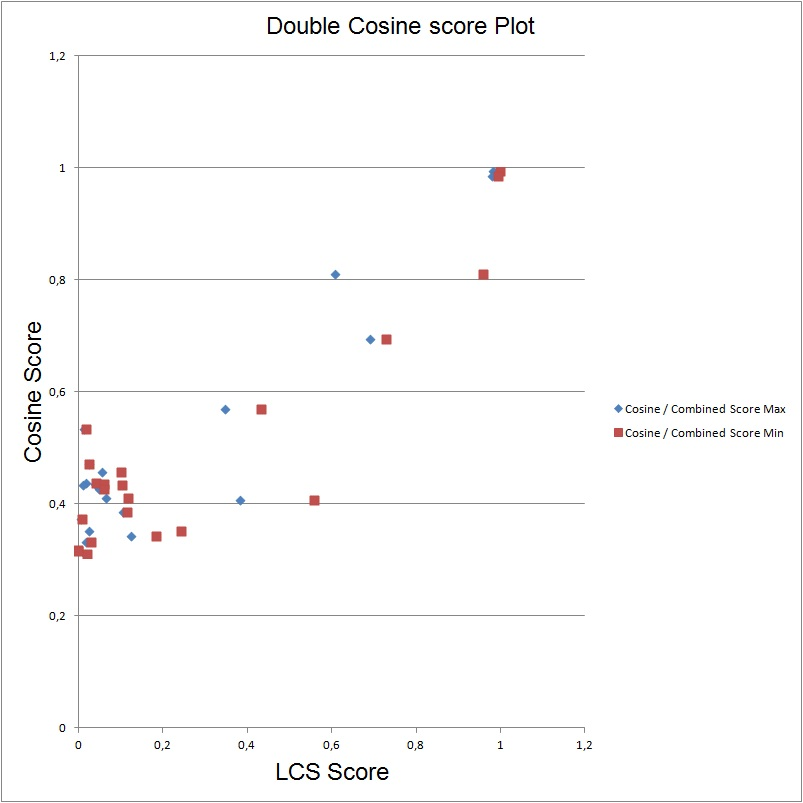
\includegraphics[scale=0.5]{figures/JPPOLCosineLCSMin}
	\caption{A plot showing the Cosine / LCS score (based off the longest article length - the blue dots) and the Cosine / LCS score (based off the shortest article length - the red squares).}
		\label{MinScore}
\end{figure}

When evaluating the figure ~\ref{JPPOLScoreGraph} we can start with looking at the first two collections of scores (comparisons \textit{e410559e / e4105525} and \textit{e410559d / e410551d}). Both comparisons have high scores in all columns. We note that the basic LCS scores around half as high as the scores for the two modified LCS scores. For the rest of this thesis I will disregard the scores produced by the basic LCS, as it holds no meaningful data when trying to find article duplicates. The length of the four articles in the comparisons is around the same length, meaning both of the LCS scores is more or less equally high.

<INDSÆT BILLEDE AF MATCHES!>S

\section{Weighing the Scores}

In combination the two sets of scores can draw us a more detailed picture, one that to a higher degree of confidence call tell about any relations between two articles. To try and break scores into something that is able to be defined, the following enums have been created, and called \textit{'Match Groups'}:

\begin{itemize}
\item \textbf{Match:} The comparison is to a high degree a perfect match, meaning that the two articles being compared have a lot of text in common, scores high with the algorithms and is somewhat similar in length.
\item \textbf{Partial Match:} This label would be a applied to a comparison, where only parts of the articles are shared, or that one article is a good deal shorter than the other, but scores highly in LCS. It would be considered an article excerpt.
\item \textbf{Same Content:} For comparisons with relative high Cosine scores, but somewhat low LCS scores, we can sometimes talk about the articles deal with the same topic, but without sharing much text. 
\item \textbf{Low Score Match:} Applying this label to a comparison would indicate that either one or both article are very short in length, can have a relative high Cosine score, but will have a high LCS score. It will indicate that the comparison most have a lot in common, but will maybe not contain much article text of much value.
\item \textbf{No Match:} When both algorithms scores low for a comparison, there is grounds to dismiss the comparison as a match. The articles will not have many sentences or special words in common.
\end{itemize}

The following table was created in order to try and give some weight to the scores. This could then be used in the program for score evaluation. The weight would be a factor that could be multiplied to the scores the algorithms produced in order to emphasize the result. These score weightings is based of tests that was done during the project.

\begin{table}
\begin{center}
	\begin{tabular}{l | c | c | c | c | c | c | c | c | c | c | r}
		    & 0.0 & 0.1 & 0.2 & 0.3 & 0.4 & 0.5 & 0.6 & 0.7 & 0.8 & 0.9 & 1.0\\ \hline
		0.0 & 0.01 & 0.01 & 0.01 & 0.01 & 0.01 & 0.01 & 0.01 & 0.01 & 0.01 & 0.01 & 0.01\\ \hline
		0.1 & 0.01 & 0.01 & 0.01 & 0.01 & 0.01 & 0.01 & 0.05 & 0.2 & 0.4 & 0.6 & 0.8\\ \hline
		0.2 & 0.01 & 0.01 & 0.05 & 0.1 & 0.1 & 0.1 & 0.3 & 0.5 & 0.6 & 0.8 & 0.85\\ \hline
		0.3 & 0.01 & 0.05 & 0.1 & 0.1 & 0.1 & 0.2 & 0.4 & 0.55 & 0.7 & 0.85 & 0.9\\ \hline
		0.4 & 0.01 & 0.05 & 0.1 & 0.1 & 0.1 & 0.2 & 0.4 & 0.6 & 0.75 & 0.85 & 0.95\\ \hline
		0.5 & 0.01 & 0.05 & 0.1 & 0.2 & 0.3 & 0.4 & 0.5 & 0.65 & 0.8 & 0.9 & 1.0\\ \hline
		0.6 & 0.01 & 0.07 & 0.1 & 0.2 & 0.4 & 0.5 & 0.6 & 0.7 & 0.85 & 0.9 & 1.0\\ \hline
		0.7 & 0.01 & 0.1 & 0.2 & 0.4 & 0.4 & 0.5 & 0.7 & 0.8 & 0.9 & 1.0 & 1.0\\ \hline
		0.8 & 0.01 & 0.1 & 0.4 & 0.6 & 0.7 & 0.8 & 0.8 & 0.9 & 1.0 & 1.0 & 1.0\\ \hline
		0.9 & 0.01 & 0.1 & 0.7 & 0.7 & 0.8 & 0.8 & 0.9 & 1.0 & 1.0 & 1.0 & 1.0\\ \hline
		1.0 & 0.05 & 0.2 & 0.8 & 0.8 & 0.9 & 0.9 & 1.0 & 1.0 & 1.0 & 1.0 & 1.0\\ \hline
	\end{tabular}
\end{center}
\caption{Score weights. The cosine score is the top most row and LCS score is the leftmost x axis. The weights indicates to what extend that articles have something in common. A low score would mean that the combination of Cosine and LCS score indicates that there is a low chance of any relation between the articles, a high score would mean the opposite. (File: Score Weight.xlsx)} \label{ScoreWeights}
\end{table}

The table ~\ref{ScoreWeights} would be an immediate indication how related two articles are, but we do also need to take another parameter into account, this being the length of the articles. A perfect match comparisons would occur when two articles of the same length and scoring close to 1.0 in both algorithms, but if two articles have a big difference in length that could affect the algorithm scores in a way that might not apply the right label when placing a comparison in a match group. The following enums was created to try and categorize articles by their length:

\begin{table}
\begin{center}
	\begin{tabular}{l | c}
	Very Short & x < 300\\ \hline
	Short & x $\geq$ 300 $\bigwedge$ x < 500\\ \hline
	Medium & x $\geq$ 500 $\bigwedge$ x < 800\\ \hline
	Long & x $\geq$ 800 $\bigwedge$ x < 1200\\ \hline
	Very Long & x $\geq$ 1200\\ \hline
	\end{tabular}
\end{center}
\caption{Enums describing article length. X is the length of the article in characters and the values it is being compared with is the article length.}
\end{table}





